%% ------------------------------------------------------------------------- %%n
\chapter{Introdução}
\label{cap:introducao}


\section{Contexto}
\label{sec:intro_contexto}



O estudo de Plâncton é de grande importância na comunidade científica, principalmente na oceanografia. O nome plâncton vem do Grego planktos e significa errante, que vaga ou flutua. Caracteriza-se, assim, por organismos planctônicos os que não possuem o poder de locomoção suficiente para evitar o transporte passivo pelas massas de água [\cite{ciotti2015vida, calazans2011organismos}].  A importância do estudo dessas criaturas se dá não somente por serem responsáveis por terem papel fundamental no ciclo de carbono, com cerca de 45\% do oxigênio produzido mundialmente [\cite{brierleyplankton}],  através da fotossíntese do fitoplâncton, mas também pela grande diversidade de classes e de características como forma, tamanho e até da natureza do local de coleta [\cite{calazans2011organismos}]. 

O plâncton é taxonomicamente diverso [\cite{brierleyplankton}]. Dentre os grupos temos o fitoplâncton (plantas), o zooplâncton (animais), o bacterioplâncton (bactérias e algas cianobactérias) e o virioplâncton (vírus aquáticos). Embora possam existir tamanhos maiores, a maioria deles são muito pequenos, variando de alguns micrômetros a 5 mm de comprimento. Além disso, existem muitas maneiras de classificar esses organismos, como em função do seu tamanho ou aspectos ecológicos [\cite{calazans2011organismos}].


A amostragem de criaturas marítimas é datada desde 1829, quando Thompson utilizou uma rede para coletar larvas de crustáceos e de cracas [\cite{brierleyplankton}]. Mas foi Victor Hensen, em 1887, o primeiro pesquisador a desenvolver, de fato, um sistema para coleta de amostras de plâncton [\cite{benfield2007rapid, wiebe2003hensen, allen1919contribution}]. Naquela época estavam interessados em responder três questões fundamentais: i) quais organismos planctônicos estão presentes no mar? ii) quantos de cada tipo estão presentes? e iii) como a composição de plâncton muda com o passar do tempo?  [\cite{benfield2007rapid}]. Essas questões continuam atuais e graças ao avanço de sistemas e equipamentos de coleta, assim como de técnicas computacionais, há um grande esforço científico para responder à essas perguntas.


Ao longo dos anos, visando o estudo desses microrganismos, foram desenvolvidas diversas maneiras de se fazer a amostragem de plâncton como, através de garrafas, redes, bombas de sucção e sistemas ópticos [\cite{calazans2011organismos}]. A figura~\ref{fig:amostragem_planctons} mostra um exemplo de uma rede planctônica. É interessante notar que nos últimos anos houve uma proliferação em sistemas ópticos. Esses sistemas permitem, por exemplo, que algumas espécies de plânctons, por serem muito delicadas, possam ser preservadas e ter suas imagens capturadas, o que nem sempre é possível com outras técnicas [\cite{benfield2007rapid}].


\begin{figure}
  \centering
  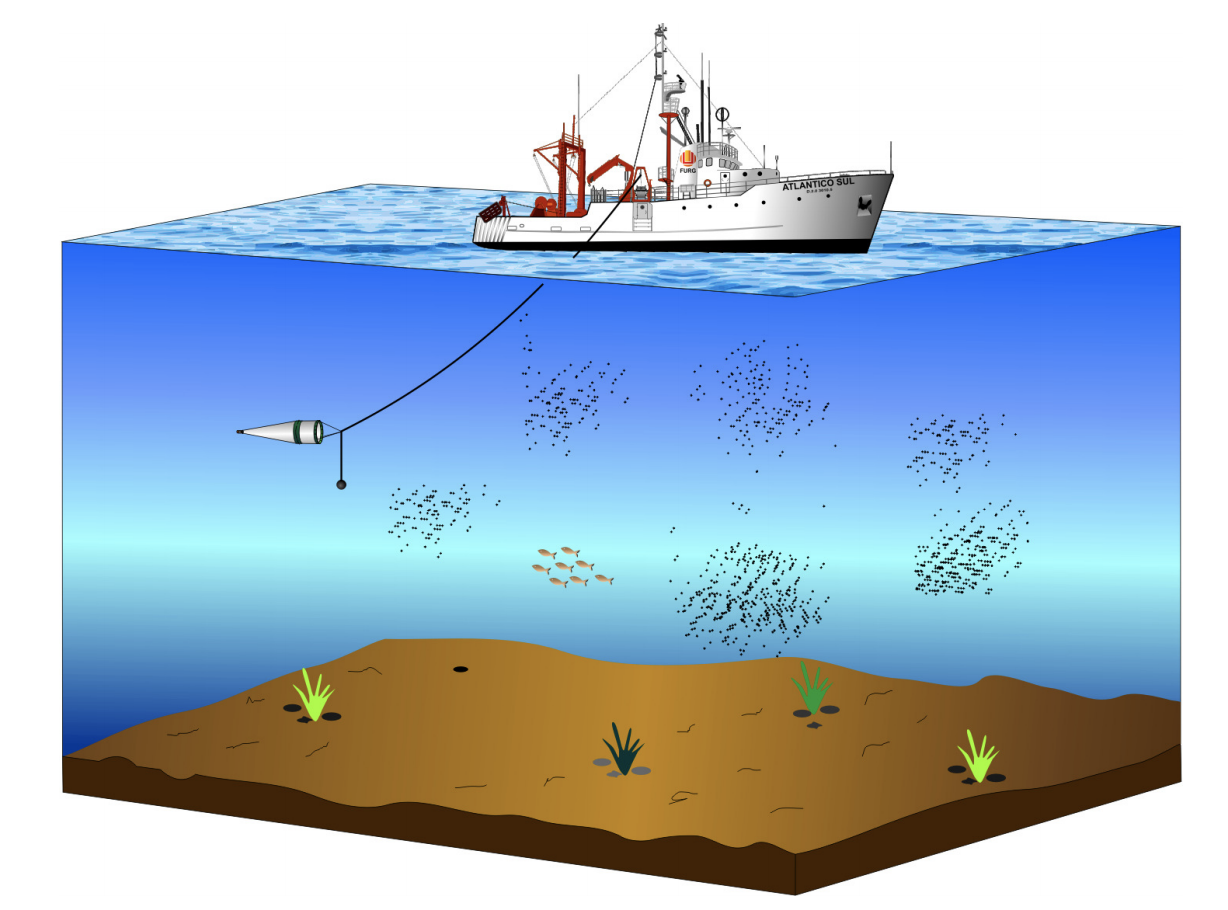
\includegraphics[width=.8\textwidth]{figures/amostragem_planctons.png}
  \caption{Rede Planctônica (Calazans, 2011)}
  \label{fig:amostragem_planctons}
\end{figure}


\section{Problema}
\label{sec:intro_problema}

Após a fase de coleta, através de sistemas ópticos, imagens de milhares de plâncton podem ser obtidas. Uma importante tarefa relacionada ao processamento e análise dessas imagens é a identificação, por exemplo, da espécie de plâncton, tarefa comumente conhecida como classificação. \NINA{Esta tarefa requer em geral conhecimentos específicos da área e portanto a atuação de um profissional especialista é necessária. Além disso, devido à grande quantidade de imagens, a realização manual dessa tarefa torna-se inviável. Diante desse quadro, as abordagens modernas utilizadas nessa tarefa consistem em automatizar a classificação por meio do emprego de técnicas de aprendizado de máquina,} e em particular, as técnicas de aprendizado supervisionado [\cite{jeffries1980computer, jeffries1984automated, berman1990image, tang1998automatic, luo2003learning, davis2004real, grosjean2004enumeration, luo2005active, hu2005automatic, blaschko2005automatic, hu2006accurate, sosik2007automated, bell2008assessment, soh2008segmentation, al2016plankton, luo2017automated, al2018intelligent}].


\NINA{As técnicas de aprendizado supervisionado geram algoritmos, também denominados classificadores, que, dada uma imagem a ser classificada, devolvem um rótulo de classe que corresponde à identificação do organismo presente na imagem. Para que seja possível gerar um classificador é necessário um conjunto de dados previamente rotulados, os chamados conjuntos de treinamento. Esse conjunto é utilizado na fase de treinamento, que é o processo de ajustes dos parâmetros de um algoritmo de aprendizado. O treinamento bem sucedido gera classificadores que são capazes não apenas de "imitar" a relação instância-classe nas amostras presentes no conjunto de treinamento mas que são capazes de extrapolar esse comportamento para instâncias novas, previamente não observadas. O conjunto de treinamento é criado em geral a partir da rotulação manual de uma grande quantidade de instâncias, em geral selecionadas arbitrariamente, e é considerada uma tarefa de custo elevado (pois depende muitas vezes de especialistas com conhecimentos sobre o domínio dos dados). Os classificadores gerados podem ser utilizados posteriormente para classificar um número arbitrário de novas instâncias~\citep{jeffries1980computer, jeffries1984automated, berman1990image, tang1998automatic}.} 

\NINA{Em muitas situações, um classificador gerado a partir deste processo não apresenta desempenho satisfatório ou seu desempenho degrada à medida que as características das imagens coletadas sofrem alterações. Por exemplo, as características das imagens de plâncton podem variar, dependendo do local ou da época, ou ainda, do tipo de equipamento utilizado na coleta. Nessas situações, torna-se necessário melhorar ou redesenhar os classificadores. Um procedimento ingênuo consiste em simplesmente preparar um novo conjunto de treinamento e refazer o treinamento. Esse processo possui alto custo e é demorado, não sendo prático na maioria das situações. Motivado por esses tipos de limitações, muita pesquisa tem sido feita para lidar com essas situações nas quais  há a abundância de dados não rotulados, mas cujo custo de rotulação é elevado.}




\section{Proposta}
\label{sec:intro_proposta}


As técnicas na área de aprendizado de máquina conhecidas na literatura para se trabalhar com situações de amostras abundantes, porém com uma quantidade nula ou limitada de dados rotulados concentram-se nas subáreas de Aprendizado Ativo~\cite{settles2014active} e aprendizado semi-supervisionado~\cite{}. \NINA{O aprendizado ativo consiste de um método de aprendizado iterativo, no qual o classificador é gradativamente melhorado incorporando-se novos dados informativos ao conjunto de treinamento. A escolha dos dados informativos é realizada pelo próprio algoritmo e um oráculo é consultado para confirmar ou corrigir o rótulo dos dados escolhidos. Na prática, o papel de oráculo pode ser desempenhado por um humano.}  Isso é extremamente importante em problemas \NINA{nos quais a rotulação é custosa} [\cite{saito2014active}], como no caso de classificação de plâncton. Além disso, estudos mostram que a inclusão de conhecimento humano especializado pode aumentar a acurácia dos modelos [\cite{benfield2007rapid}].

Trabalhos recentes na área de aprendizado ativo têm como objetivo permitir um papel mais ativo ao humano, em contraste aos trabalhos pioneiros no qual o papel do oráculo é totalmente passivo. Essa não é uma questão nova [\cite{castro2009human, dasgupta2011two}] e estudos demonstram resultados positivos podem ser alcançados com a intersecção do aprendizado ativo com a ciência cognitiva [\cite{kottke2018other}]. Uma maneira aliar aprendizado ativo e percepção cognitiva é por meio da interação do usuário humano com a visualização de dados [\cite{yang2018visually, bernard2018comparing, weigl2016mapview}].  


A proposta desta dissertação consiste em desenvolver um método efetivo para a rotulação e a classificação de imagens de plâncton, usando técnicas de aprendizado ativo, aprendizado semi-supervisionado e interação ativa de usuários. Para tanto, a ideia central consiste em encontrarmos boas representações das imagens, representações que capturem similaridades entre os organismos, formas interessantes de visualizar as estruturas e padrões presentes no conjunto de dados (através de projeções 2D ou galeria de imagens), juntamente com mecanismos de interação nos quais o usuário especialista poderá selecionar amostras e informar os respectivos  rótulos. As imagens rotuladas podem, assim, ser utilizadas no framework de aprendizado ativo para a produção de um classificador e esse processo, que realizará a propagação de rótulos, teria como objetivo agilizar a rotulação das imagens restantes. O objetivo principal é atingir uma boa taxa de acerto com o menor número possível de interações por parte do usuário. Em outras palavras, ao invés de rotular uma grande quantidade de dados de forma arbitrária, o usuário especialista rotularia uma quantidade menor de dados, selecionados cuidadosamente ou pelo algoritmo ou pelo próprio usuário.

Para validar o método a ser proposto, pretende-se utilizar como baseline para comparação o aprendizado ativo clássico, no qual o usuário interage apenas como um oráculo passivo. Também pretendemos fazer comparações com o treinamento realizado a partir de seleção aleatória de dados, uma forma de validação normalmente utilizada em trabalhos da área. No método a ser desenvolvido, espera-se agregar possibilidades de interação mais ativa por parte do usuário, nas quais o usuário poderá escolher quais amostras valem a penas ser rotuladas. Conjectura-se que, com um usuário desempenhando um papel mais ativo, um número menor de iterações seja suficiente para se obter classificadores com desempenho similar ao obtido com o framework clássico (oráculo passivo) de aprendizado ativo.

%\section{Trabalhos Relacionados}
%\label{sec:intro_relacionados}

%To do: citar trabalhos relacionados, principalmente nos últimos anos. Falar, por exemplo, do trabalho da Priscila. 


\section{Organização}
\label{sec:intro_organizacao}

Este texto de qualificação está organizado da seguinte maneira: o capítulo~\ref{cap:aprendizado_ativo} faz uma revisão de conceitos e fundamentos de Aprendizado Ativo e comenta a respeito das principais limitações e desafios. O capítulo~\ref{cap:Proposta} detalha a proposta deste trabalho. O capítulo~\ref{cap:Experimentos_Resultados} mostra alguns experimentos e resultados preliminares, enquanto o último capítulo descreve um plano de trabalho e respectivo cronograma.